%!TEX root = ../bare_jrnl.tex

\section{Exploration on Human Occupancy Behaviour}
\label{sec:exploration}

Up to this point, this paper has been concerned with Bayesian methods for estimating count data. We demonstrated the power of these methods by estimating human occupancy counts given unreliable robot sensors. In this section, we use the predictions made by our methods to drive robotic \emph{exploration} to detect humans. In particular, our aim is to create a policy which takes the robot to the regions where there are the most people present in the long run, i.e.\ where the aggregate level of human occupancy is highest. 

\subsection*{Exploration Models}



Planning to optimise a value estimated with a learnt model (e.g.~the expected number of people present estimated with a POPP filter), where the model is built from data gathered online, is an instance of an \emph{exploration-exploitation} problem.
% 
Exploration-exploitation problems arise when an agent, in this scenario a mobile robot, does not fully understand the process it is trying to control. At any time, the agent can choose to explore or to exploit its model of the process.
Exploration allows the agent to better understand the process by gathering more data, leading to a better action later on, but sacrificing short-term reward.
Exploitation allows the agent to  leverage what it already understands about the process to gain reward immediately, but risks following a policy that might be suboptimal. 
% 
In our problem, visiting a region both explores and exploits it. Our decision problem is a choice between which regions to visit next, as each region will offer the robot different exploration-exploitation opportunities.

% In each time the robot has a choice between many actions, each of which both explores and exploits a certain place, but to varying degrees. As its goal is to maximise the reward gathered–as in getting as much data on human activities (by seeing as many humans) as possible–given its limited operational life, it is preferable to have a policy that is as near optimal as possible.

While exploration-exploitation problems in reinforcement learning are typically intractable, there are well known approximate approaches that are quick to compute~\cite{wyatt1998exploration, 1413255, AUDIBERT20091876}. One such approach is to use the upper bound of a probability distribution over the quantity being maximised. This causes the decision-making agent to exploit high-scoring, certain estimates, and explore highly uncertain estimates. In our case we use an upper bound on the arrival rate ($\lambda$) of a Poisson process ($\lambda_{UB}$) to choose the region for the robot to visit next. The upper bound of the probability interval of the arrival rate of a Poisson process is calculated as follows:

\begin{equation}
	\label{eq:upper_bound_exploration}
	\begin{tabular}{r@{ = }l}
	$\lambda_{UB}(t_i, t_j)$ & $\displaystyle \int_{t_i}^{t_j} CDF^{-1}(\% = 0.95 \mid \alpha_t, \beta_t)~dt$\\ [1ex]
	\end{tabular}
\end{equation}

\noindent with $\lambda_{UB}(t_i, t_j)$ as the upper bound of $\lambda$ within time $t_i$ and $t_j$, $i, j \in \{1, \ldots, \Delta\}$, and $CDF^{-1}$ as the inverse of the cumulative density function of a gamma distribution. Given the upper bounds $\lambda^{r}_{UB}(t_i, t_j)$ for each region $r$ from the set of all regions $R$, the region to be visited between time $t_i$ and $t_j$ is chosen by:

\begin{equation}
\label{eq:choosing_place}
\underset{r \in \mathcal R}{\arg\max}~\lambda^{r}_{UB}(t_i, t_j)
\end{equation}
\noindent Figure~\ref{fig:map_vs_ub} depicts a comparison between the MAP hypothesis estimate and the upper bound estimate of a Poisson process.

\begin{figure}[t!]
	\centering
	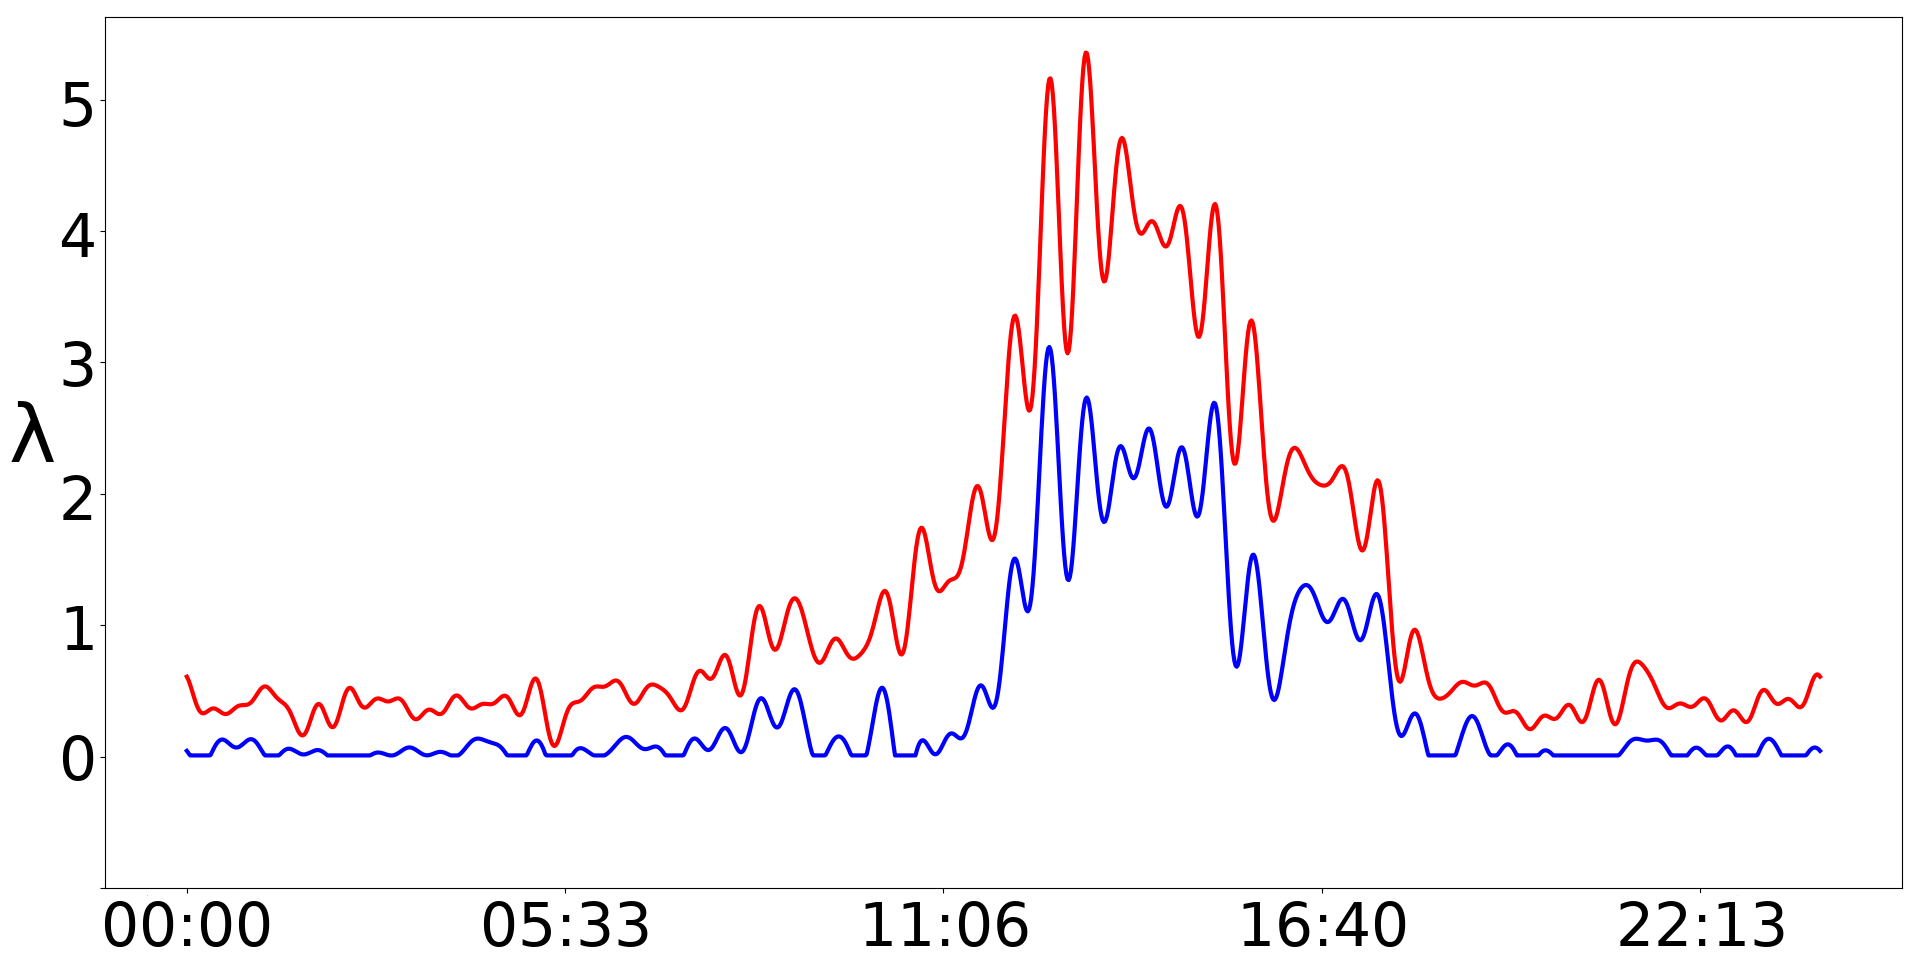
\includegraphics[width=0.5\textwidth]{./figures/map_vs_ub.png}
	\caption{A periodic Poisson process of region 9 (see Figure \ref{fig:map_popp_independent_test}) represented by its MAP hypothesis (blue line) and its upper bound of the probability interval (red line).}
	\label{fig:map_vs_ub}
\end{figure}


To tie the estimate of a particular Poisson process over a time interval to data collected previously, as in Section~\ref{sec:evareal} we assume that human presence in each region follows a \emph{periodic} Poisson process with daily periodicity. This allows us to regularise, and fill missing data, across the point estimates of upper bounds using methods based on the Fourier transform.  This exploits assumptions and algorithms introduced in our prior work. In particular, the series of upper bounds $\lambda_{UB}(t_i, t_j)$ are encoded and extracted via spectral analysis with the $l$-AAM technique described in~\cite{jovan_iros16}. Algorithm 2 depicts the process of computing the upper bound of $\lambda$ of a Poisson process and applying spectral analysis to it. The plot in Fig.~\ref{fig:map_vs_ub} shows the effects of the spectral processing. We use this approach with upper bounds produced by our previously presented estimators: FOPP, POPP, and POPP-Beta. 

\begin{figure}[t!]
	\begin{center}
		\begin{tabular*}{0.5\textwidth}{l @{\extracolsep{\fill}}}
			\hline
			\textbf{l-AAM} \textrm{\cite{jovan_iros16}} \\
			\hline
			\textbf{Input:} $x_1, \ldots, x_n$: input signal, \\
			\hspace{0.3cm} total: maximum total frequency \\
			\textbf{Output:} $\mathcal S$: a collection of $(s, p, f)$ \\
			\textbf{Procedure:}\\
			\hspace{0.3cm} 1. Init. k $\leftarrow$ 0 \\
			\hspace{0.3cm} // Get frequency $0$ with Discrete Fourier Transform \\
			\hspace{0.3cm} 2. $[s, p, f] \leftarrow DFT(x_1, \ldots, x_n)[0]$\\
			\hspace{0.3cm} 3. $\mathcal S[k] \leftarrow [s, p, f]$ \\
			\hspace{0.3cm} 4. Repeat until k $>$ total \\
			\hspace{0.7cm} $\bullet ~ k \leftarrow k + 1$ \\
			\hspace{0.7cm} // Get the frequency with the highest amplitude \\
			\hspace{0.7cm} $\bullet ~ [s, p, f] \leftarrow \argmax_s DFT(x_1, \ldots, x_n)$ \\
			\hspace{0.7cm} // Update $\mathcal S$ with frequency $f$ \\
			\hspace{0.7cm} $\bullet$ if $f \in \mathcal S$, $[s', p', f'] \leftarrow \mathcal S[k', f'=f]$ \\
			\hspace{2.5cm} $s \leftarrow s + s'$; $p \leftarrow p + p'$ \\ 
			\hspace{0.7cm} $\bullet$ $\mathcal S[k] \leftarrow [s, p, f]$ \\
			\hspace{0.7cm} // Create a cosine signal from $f$ \\
			\hspace{0.7cm} $\bullet ~ x'_1, \ldots, x'_n \leftarrow s * ~ cos(2 \pi * f + p)$ \\
			\hspace{0.7cm} // Subtract current $x_1, \ldots, x_n$ with the cosine signal \\
			\hspace{0.7cm} $\bullet ~ x_1, \ldots, x_n \leftarrow x_1, \ldots, x_n - x'_1, \ldots, x'_n$ \\
			\hline
		\end{tabular*}	
	\end{center}
\end{figure}

\begin{figure}[t!]
	\begin{center}
		\begin{tabular*}{0.5\textwidth}{l @{\extracolsep{\fill}}}
			\hline
			\textbf{Algorithm 2} \textit{Upper Bound} \\
			\hline
			\textbf{Input:} $(\alpha_1, \beta_1), \ldots, (\alpha_n, \beta_n)$: Poisson process \\
			\textbf{Output:} $\lambda^{ub}_1, \ldots, \lambda^{ub}_n$: upper bound \\
			\textbf{Procedure:}\\
			\hspace{0.3cm} 1. Init. k $\leftarrow$ 1, m $\leftarrow$ $\eta$ \\
			\hspace{0.3cm} 2. Repeat until k $>$ n \\
			\hspace{0.7cm} $\bullet ~ k \leftarrow k + 1$ \\
			\hspace{0.7cm} // Get the upper bound \\
			\hspace{0.7cm} $\bullet ~ \lambda_k \leftarrow CDF(0.95, \alpha_k, \beta_k)$ \\
			\hspace{0.3cm} // Transform $\lambda_1, \ldots, \lambda_n$ to with $l$-AAM \\
			\hspace{0.3cm} 3. $\mathcal S$ $\leftarrow$ \textbf{l-AAM}($\lambda_1, \ldots, \lambda_n$, m) \\
			\hspace{0.3cm} 5. Init. k $\leftarrow$ 0,  $\lambda^{ub}_1, \ldots, \lambda^{ub}_n \leftarrow (0, \ldots, 0)$ \\
			\hspace{0.3cm} 4. Repeat until k $>$ m \\
			\hspace{0.7cm} // Create a cosine signal from $\mathcal S[k]$ \\
			\hspace{0.7cm} $\bullet ~ [s, p, f] \leftarrow \mathcal S[k]$ \\
			\hspace{0.7cm} $\bullet ~ x_1, \ldots, x_n \leftarrow s * ~ cos(2 \pi * f + p)$ \\
			\hspace{0.7cm} // Add current $\lambda^{ub}_1, \ldots, \lambda^{ub}_n$ with the cosine signal \\
			\hspace{0.7cm} $\bullet ~ \lambda^{ub}_1, \ldots, \lambda^{ub}_n \leftarrow \lambda^{ub}_1, \ldots, \lambda^{ub}_n + x_1, \ldots, x_n$ \\
			\hline
		\end{tabular*}	
	\end{center}
\end{figure} 


\subsection*{Exploration Evaluation}

The dataset used in the previous section was collected by a mobile robot over 69 days of a real world deployment. This robot was controlled by the exploration models described above. Due to hardware failures, sensor malfunctions and other external issues, only 48 days from the dataset were usable.

Three different exploration models were applied separately during three phases of the 69 days of the deployment. All of these models used Eqn.~\ref{eq:choosing_place} to create their exploration policies. For the first 27 day phase of the deployment, the robot followed an exploration policy based on the FOPP model. This resulted in 18 days of data. From this 18 days of data, the last 3 days were used to train the sensor model needed for both the POPP and the POPP-Beta models. From day 28 to day 47, the robot followed an exploration policy according to the POPP model. This resulted in 15 days of data. Finally, from day 48 onwards, the robot followed an exploration policy according to the POPP-Beta model. This resulted in 15 days of data.
% 
%For this comparison, the last 3 days which are part of the 18 days worth of data collected by following the FOPP exploration model are included in the POPP and the POPP-Beta exploration models. This is necessary to avoid the POPP and the POPP-Beta exploration models having an advantage over the FOPP exploration model since the POPP and the POPP-Beta need a training period to construct their sensor model. Moreover,
% 
We can compare the different exploration policies on the observations the robot made during the phase each policy was active. Due to the absence of information regarding occupancy in the places that the robot did not visit, only a comparison of the positive observations can be made. 

% As a note, a positive observation is a duration when the robot observes any activity during its visit to a particular area. 

\begin{figure}[t!]
	\centering
	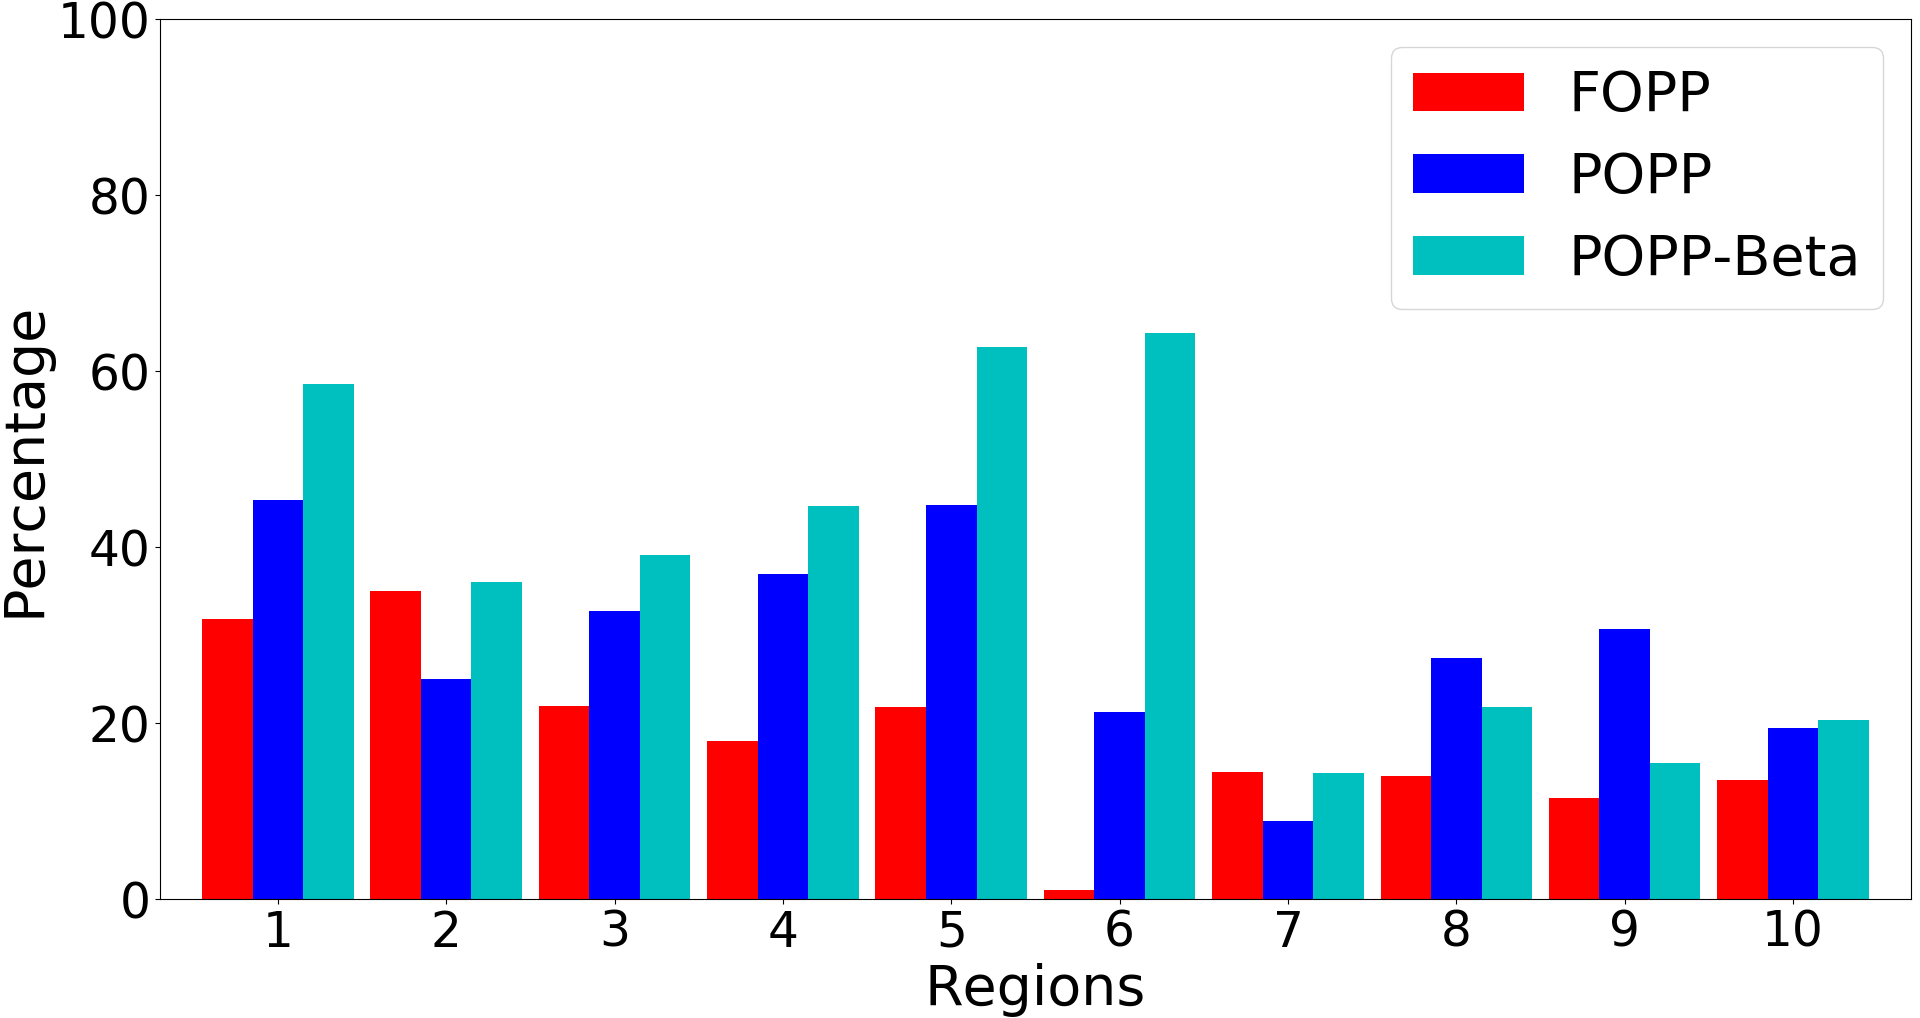
\includegraphics[width=0.5\textwidth]{./figures/exploration_percentage_region.png}
	\caption{The activity exploration percentage across areas of the environment using three different exploration models (FOPP, POPP, POPP-Beta). The percentage shows the portion of time that the robot was observing activities.}
	\label{fig:exploration_percentage_region}
\end{figure}

%\begin{figure}[t!]
%	\centering
%	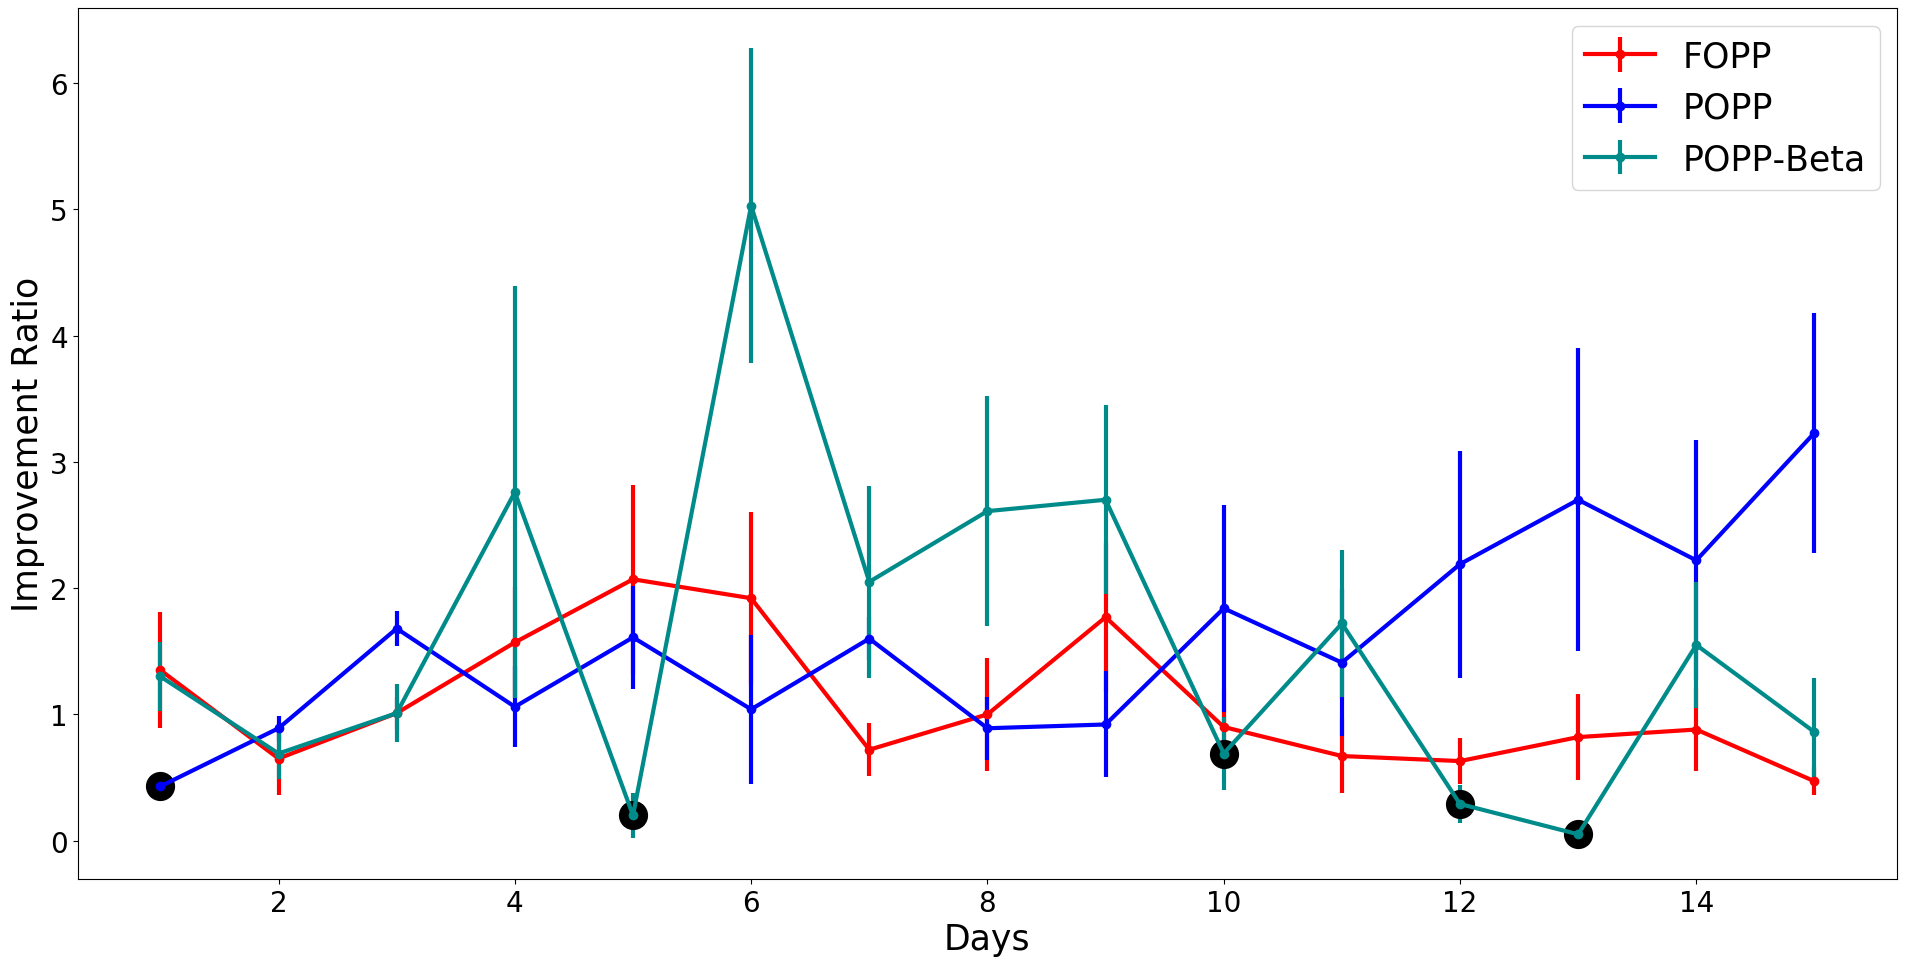
\includegraphics[width=0.5\textwidth]{./figures/exploration_improvement_ratio.png}
%	\caption{The improvement evolution of activity observation (in ratio) using three different exploration models. The average of the first three days of the number of observations on each exploration is used as the base (ratio 1.0). Black dots represent weekends the explorations were passing through.}
%	\label{fig:exploration_improvement_ratio}
%\end{figure}

%\begin{figure}[t!]
%	\centering
%	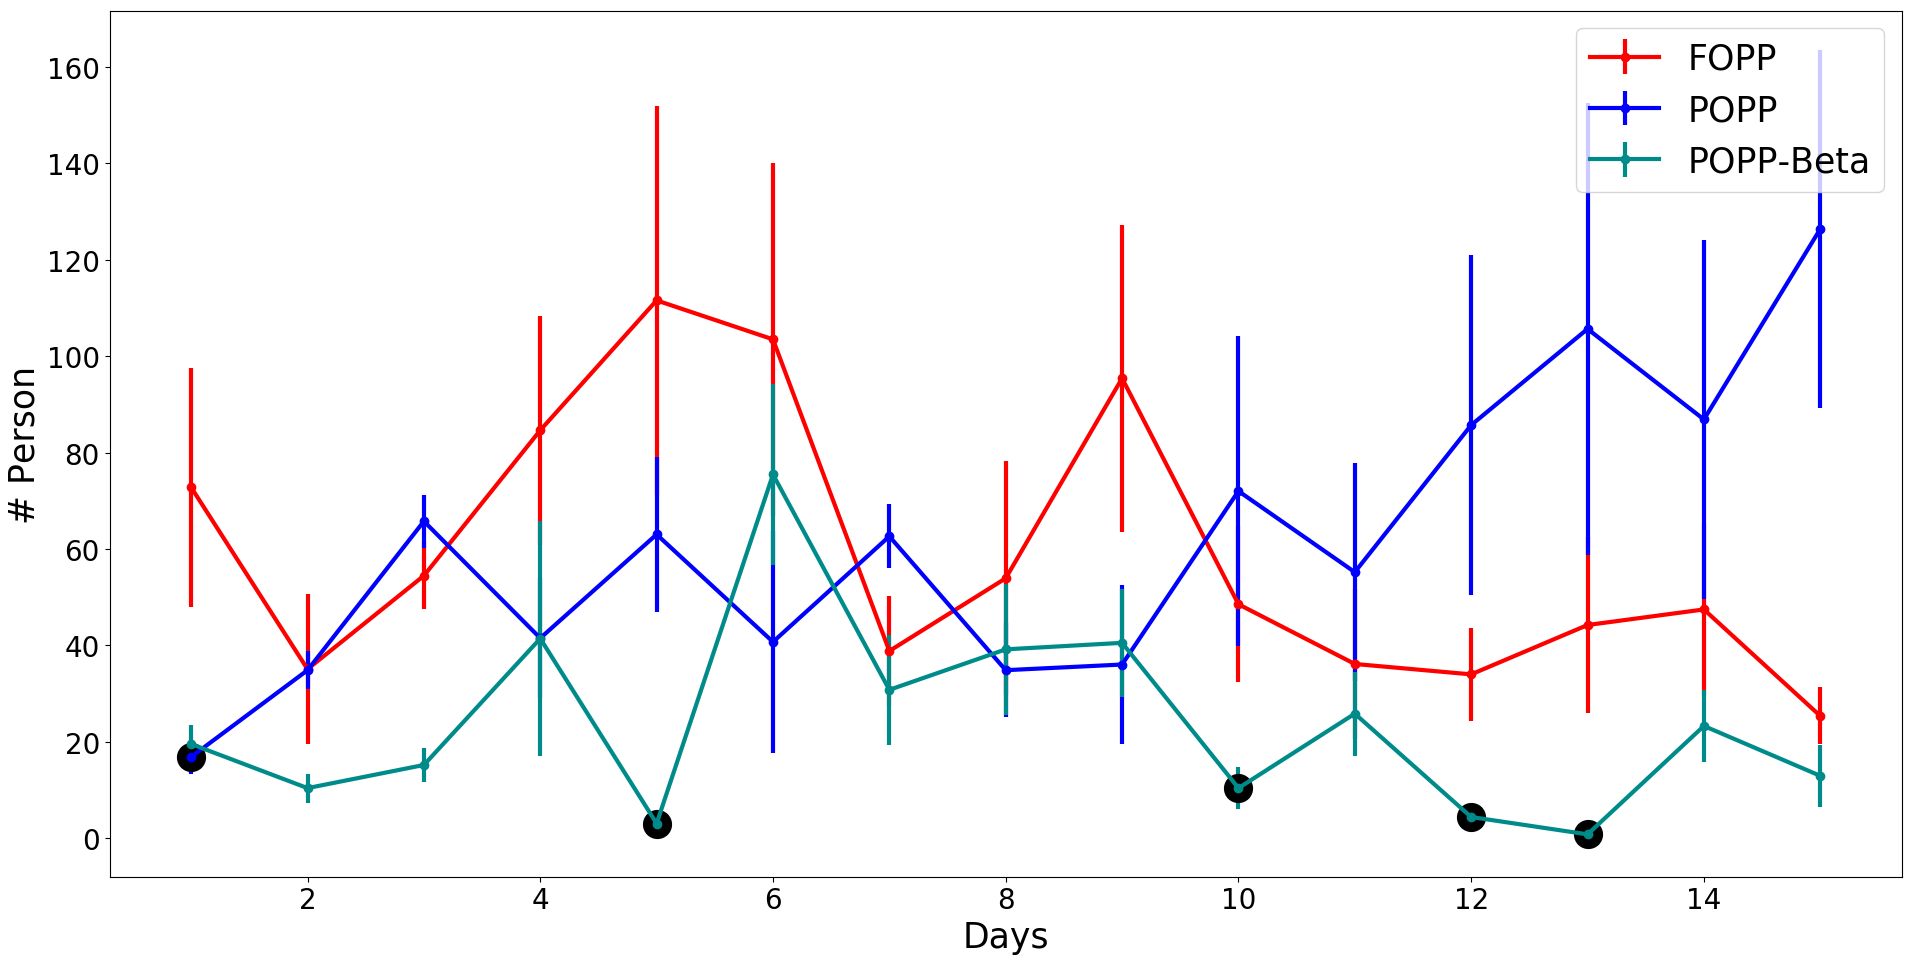
\includegraphics[width=0.5\textwidth]{./figures/exploration_number_people_across_days.png}
%	\caption{Average number of activities observed over days across regions. Black dots represent weekends the explorations were passing through.}
%	\label{fig:exploration_number_people_across_days}
%\end{figure}

\begin{figure}[t!]
	\centering
	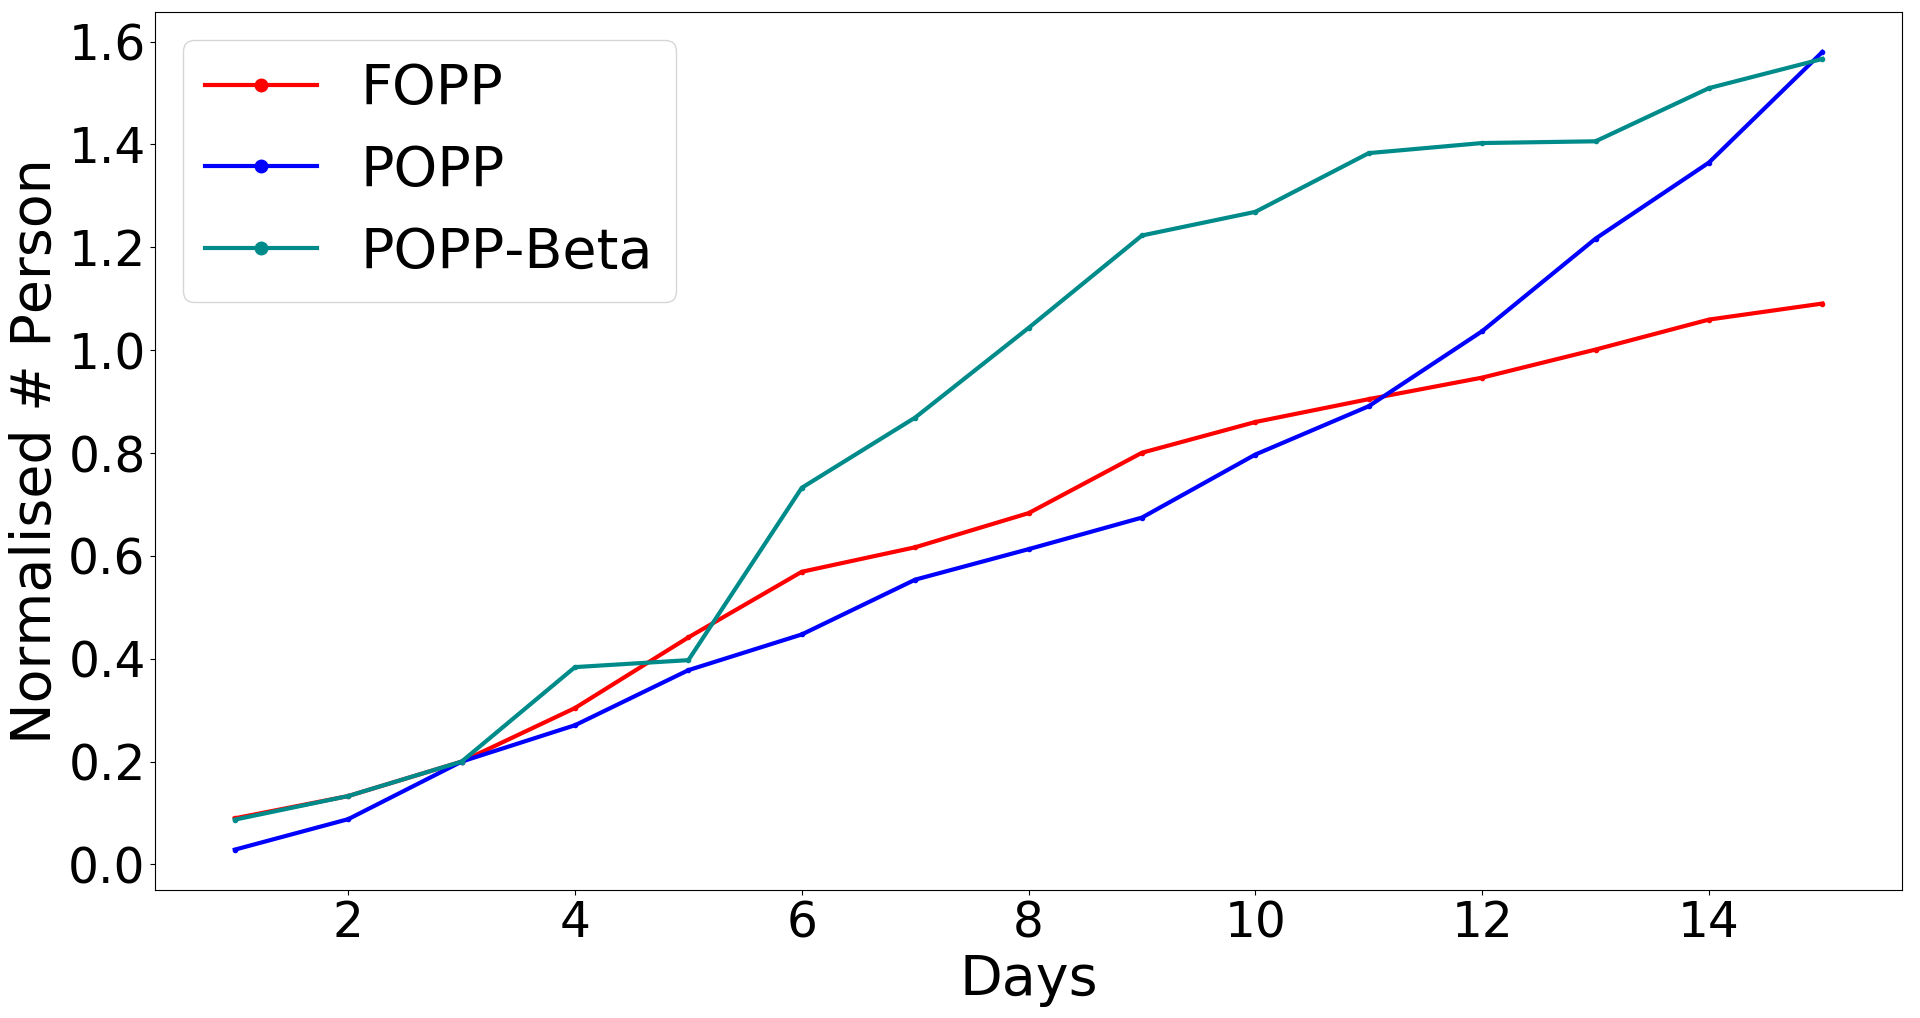
\includegraphics[width=0.5\textwidth]{./figures/exploration_number_people_across_days_normalised.png}
	\caption{The improvement ratio of activity observations during each phase of the deployment. A ratio of 1.0 means that the exploration model gives no improvement over time in finding more people.}
	\label{fig:exploration_improvement_ratio}
\end{figure}

Figure \ref{fig:exploration_percentage_region} shows the percentage of visits to each region which yielded a non-zero true count. As can be seen, the exploration policy produced by POPP-Beta has the highest proportion of such visits in many of the regions, followed by the exploration policy according to the POPP model. Recall that some regions, such as 4, 5, 6, and 7, are not densely populated with humans across time compared to other regions (such as 1, 2, 3, and 10). The POPP and POPP-Beta models, however, still managed to improve the percentage of positive observations. This shows that the models correctly predicted that people would be present in particular locations at particular times. One should note that region 6 contains vending machines which are often detected as a person by the upper body detector. This leads to the FOPP model planning to visit this particular location when no activity is taking place. The POPP and the POPP-Beta models were able to correct the miscounts occurring in region 6, providing a better estimate of the posterior over the arrival rate $\lambda$. This leads to models that better capture the true underlying process and thus support more accurate exploration-exploitation trade-offs.

% Figure \ref{fig:exploration_number_people_across_days} shows the average number of activities observed across regions on each day. 

During the first few days of each phase the above models cause the robot to primarily explore since the estimates of $\lambda$ are initially highly uncertain. We use these initial days as a baseline against which later days (featuring greater exploitation) can be compared. To do this, we divide all true counts by the sum of the true counts over the first three days. Since we have 15 days of usable data for each phase we also divide the counts by 5 such that a score of 1.0 on day 15 represents continuing to observe people at the same rate as experienced in the first 3 days. Formally, the normalised number of persons observed on day $n$ can be calculated as:

\begin{equation*}
\hat{s}(n) = \frac{\displaystyle\sum_{i=1}^{n} s(i)}{\displaystyle\sum_{i=1}^{3} s(i) * 5}
\end{equation*}

\noindent with $s(n)$ be the number of persons observed on day $n$. A score above 1.0 on day 15 shows that exploitation has led to people being observed at a greater rate than in the first 3 days. This normalisation is necessary since there were large fluctuations in the total number of people present in the robot's environment over the 10 weeks of the deployment.

% 
Figure \ref{fig:exploration_improvement_ratio} presents the cumulative normalised true counts of people observed by the robot across the three phases. This shows that exploration driven by the POPP and the POPP-Beta models improves the number of people observed during these phases. By the end of each of these two phases, the ratio is around 1.7. On the other hand, the FOPP showed a stable ratio around the baseline (1.0 at day 15), this means that the FOPP is not be able to improve the number of people observed over time. 
% 
Also note the general trend observed earlier that the approaches which represent the uncertainty in the sensor models (POPP-Beta) initially out-perform less informed approaches (POPP) until the latter have observed enough of the underlying process to compensate for training inaccuracies. 

%Unfortunately for the POPP-Beta, by looking at figure \ref{fig:exploration_improvement_ratio}, we can not conclude whether the POPP-Beta can improve the number of activities observed over time.
%We argue that this is because the exploration policy produced by the Specctral-POPP-Beta was running through several weekends. We assumed of daily periodicities for the non-homogeneous Poisson processes across regions, and the assumption was broken by running the exploration throughout weekends. This is because weekdays and weekend have different arrival rate $\lambda$. Figure \ref{fig:exploration_number_people_across_days} clearly shows how small the total activities observed during weekend compared to weekdays.